\section{Library design and implementation}
The previous chapter focused on the domain decomposition method and how to model the underlying source graph for stencil codes.
However, domain decomposition is only the initial part of this automated domain decomposition library for stencil codes.
Once the domain is decomposed additional functionalities need to be provided to make a stencil code run on a decomposed domain.

Conceptually the library can be separated into three distinct parts:
Pre-process, runtime, and post-process.
The flowchart in Fig. \ref{fig:library_flowchart} gives an abstract overview of the whole automatic domain decomposition process.

\begin{figure}
\centering
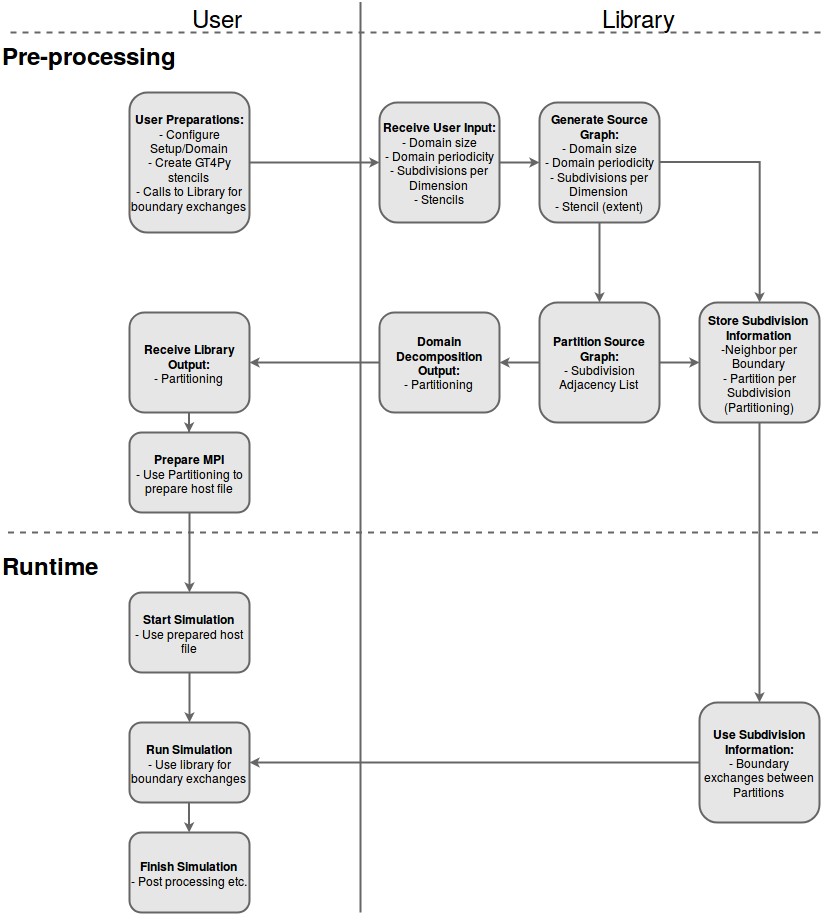
\includegraphics[width=\textwidth]{ddflowchart.png}
\caption{Schematic description of the flow for the automatic domain decomposition process.}
\label{fig:library_flowchart}
\end{figure}

The next sections will first outline the design and functionality of each of these three parts and then show and explain the user facing functions in more detail with examples.

\subsection{Design}


\subsubsection{Pre-process}
The pre-process contains functionalities needed before the main, distributed stencil computations are performed.
Specifically, the actual domain decomposition happens during the pre-process.
Therefore the pre-process contains functions to prepare the graph partitioning files, perform the actual graph partitioning, and store the results.

The design and implementation of the pre-process functions follows the descriptions of the source graph generation, and graph partitioning from the previous chapter in the Sections \ref{sec:commcost}, \ref{sec:compcost}, and \ref{sec:sourcegraphgeneration} and the pseudo-code of Algorithm \ref{alg:domaindecomposition} very closely and is therefore not repeated here.
The user-facing part of the pre-process implementation is outlined with examples in Section \ref{sec:userpreprocess}.

\subsubsection{Runtime process}
\label{sec:runtime_process}
During the runtime of a stencil computation the domain decomposition library has to manage a few tasks.
Most of them arise because once the domain is decomposed into smaller parts each of these parts needs to be managed separately.
At the same time the goal for the user facing parts of the library is to avoid adding complexity.
To achieve both these goals the runtime functions of the domain decomposition library are organized into two main classes:
The user facing \texttt{DomainDecomposition} class and the internal \texttt{DomainSubdivision} class.

The \texttt{DomainDecomposition} class holds a list of all subdivisions i.e. \texttt{DomainSubdivision} objects belonging to the partition of the corresponding MPI process.
Specifically, in the initialization of the \texttt{DomainDecomposition} class each MPI process loads the full serialized list of subdivisions from the pre-process and removes all subdivisions given to a different partition by the graph partitioning of the pre-process.

In general the purpose of the \texttt{DomainDecomposition} is mostly to hide the separate subdivisions from the user and give the user a single point of contact with the library functions.
Internally the \texttt{DomainDecomposition} contains functions that mostly just delegate function calls to all subdivisions.

The \texttt{DomainSubdivision} class in contrast is responsible for the actual stencil computation.
This includes managing and storing the fields in NumPy arrays, carrying out the GridTools4Py stencils computations, exchanging the boundaries between subdivisions, as well as applying the global boundary condition in the appropriate subdivisions.

The fields and stencils need to be managed in the \texttt{DomainSubdivision} class because each subdivision needs its own fields and each GridTools4Py stencil has to be instantiated with a specific field.

The hierarchical structure and the functions that are delegated between these two classes is illustrated in Fig. \ref{fig:classes_chart}.

\begin{figure}
\centering
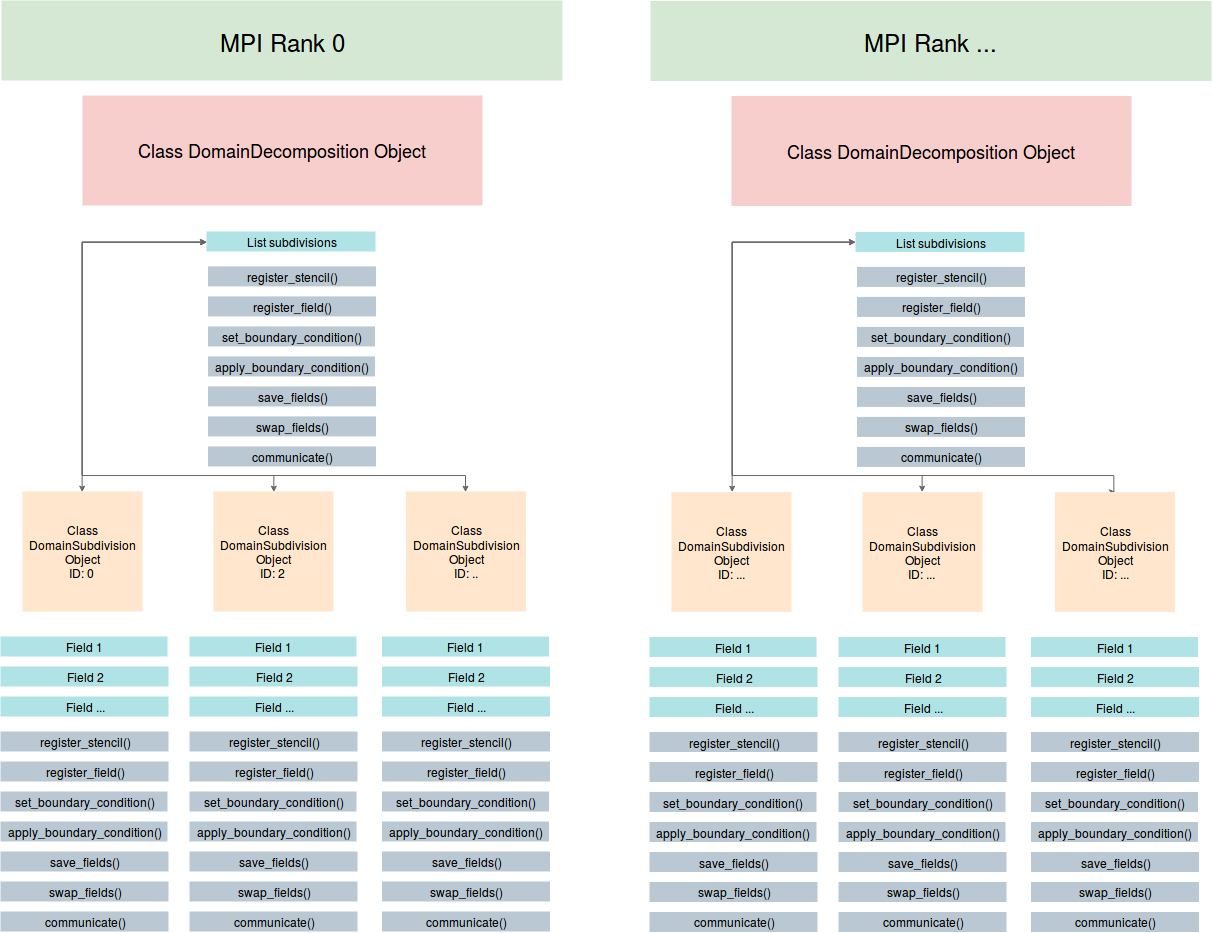
\includegraphics[width=0.85\textwidth]{Classes_Delegation.png}
\caption{Hierarchical structure of the main components of the runtime classes of the domain decomposition library.}
\label{fig:classes_chart}
\end{figure}

The next paragraphs will describe some implementation details of the main runtime functionalities.

\paragraph{Field registration } replaces for the user the usual call to NumPy to instantiate an array for a field.
The subdivisions store fields as a dictionary containing the name of the field as the key and the array itself as the value.
The name of the field needs to be stored alongside the array because of the indirection introduced by the domain decomposition.
The indirection here is that the user wants to operate on a single array as the field while the decomposed domain consists of many arrays for each field.
Storing the name of the field in addition to the NumPy arrays is a necessary compromise between these two aspects.
Basically, this addition allows the user to refer to a field by its name in many functions where in the original code it would return to the NumPy array of the field.

Internally the field registration delegates the array instantiation to the subdivisions and also calls the internal functions to setup the NumPy views to define the halo region used in the communication function.
The creation of these boundary views is done during field registration because this is the first time the subdivisions get the name of a field as input and it is assumed that any field might need to communicate its boundary with the neighboring subdivisions.

The following boundary views are created:

The NumPy view called \texttt{recv\_slices} stores the indices of the halo region in each direction.
The indices of the halo region in a given direction are $0:hs$ for negative directions where $hs$ is the size of the halo in the corresponding direction and $-hs:$ for positive directions.
Note that the various $hs$ in these descriptions can refer to different values if the halo size varies between dimensions and directions.
The indices in the two dimensions not corresponding to the direction are both $-hs:hs$.
The order of directions for \texttt{recv\_slices} is negative x-direction, positive x-direction, negative y-direction, positive y-direction, negative z-direction, and positive z-direction.

The next NumPy view called \texttt{send\_slices} stores the indices of the outermost regions neighboring the halo regions.
These are the boundary values that are the halo region of the neighboring subdivision.
For these send regions the indices in a given direction are $hs:hs+hs$ for negative directions and $-hs -hs:-hs$ for positive directions.
Indices in the two non-direction dimensions are again $-hs:hs$.
The order of directions for \texttt{send\_slices} is negative x-direction, positive x-direction, negative y-direction, positive y-direction, negative z-direction, and positive z-direction.

The third NumPy view is called \texttt{get\_local} and stores the the same indices as \texttt{send\_slices} in a different order.
The order is positive x-direction, negative x-direction, positive y-direction, negative y-direction, positive z-direction, and negative z-direction.
This NumPy view is used for the local communication between subdivisions in the same partition.
The reason for the difference in order is described in more details in the communication paragraph.

The last NumPy view is called \texttt{get\_global} and combines the same indices as the last two NumPy views with the global coordinates of the subdivision.
This NumPy view is only used if the global boundary condition is provided in a single file and therefore is not feasible for large computational domains.

%In all the mentioned NumPy views care has to be taken during the index calculations in the case of halo size $0$.
%NumPy views that have indices like $0:0$ result in empty NumPy arrays instead of valid halo regions.
%Therefore, in the index calculations $0$ halo sizes have to be replaced with \texttt{None}.
%Using \texttt{None} results in valid NumPy views instead of empty NumPy arrays.
%However, the communication functions described later should always catch halo sizes of $0$ and therefore these NumPy views should never actually be used.

\paragraph{Stencil registration } can be done once all the fields used in the stencil have been registered.
Stencil registration involves the same keywords that instantiation of a GridTools4Py stencil would.
With the exception of the \textit{domain} keyword which is ignored since the stencil domain depends on the subdivision size and the stencils halo and not user input.
However an additional keyword \textit{reductions} allows the user to limit the stencil domain if only a smaller part of the domain should be used.

Otherwise the most obvious difference is that instead of NumPy arrays directly the \textit{inputs} and \textit{outputs} keywords need to be provided with the field names instead since every subdivision has their own NumPy array to give to the GridTools4Py stencil.

To keep the handling of GridTools4Py stencils similar to non-decomposed code the \texttt{register\_field()} function returns a single object that has a \texttt{compute()} function that can be called after instantiation.
For the domain decomposition library this object is not the GridTool4Py stencil directly but instead an object of the small internal helper class \texttt{DomainDecompositionStencil} which does nothing more than store the subdivisions stencils in a list and provide a \texttt{compute()} function to delegate to the subdivisions \texttt{compute()} functions.

\paragraph{Communicate } functions are needed because the subdivisions of the domain need to exchange their boundaries with each other in between computations.
For the user this function needs to be called every time the values of a field need to be up to date i.e. in most cases after or just before the stencil computation.
Internally this function encompasses all functions updating the halo region of a field or a list of fields.
Specifically, the \texttt{DomainDecomposition.communicate()} function delegates to each \texttt{DomainSubdivision.communicate()} function which in turn calls either two-way or one-way communication functions depending on the optional flag.
Additionally, both the two-way and one-way communication have to handle neighboring subdivisions being in the same partition by calling a function to handle local communication.

Both the two-way and the one-way communication function are designed to follow the same procedure.
Section \ref{sec:onesided} gives more details on the differences for the MPI one-sided approach.
The communication procedure iterates over each direction sequentially, but for the two-way communication non-blocking send and receive functions are used so that the communication of the second direction can start before the communication of the first direction is finished.

For each direction the communication function first checks if it is at the global boundary, because the global boundary is handled in its own function.
Afterwards, the communication function checks if the neighbor in the given direction belongs to the same partition and if yes calls the local communication function.
Otherwise the external communication functions are called.
For non-blocking two-way communication the processors with an even MPI rank send first and receive second, while processors with an odd MPI rank receive first and send second.
This is done to avoid the situation where two processors both wait to receive from each other.

Local communication is just a copy between \texttt{DomainSubdivision} fields.
To copy the boundary a NumPy view of the halo region to receive into and a NumPy view to access the boundary are used.
The halo region NumPy view is the same for local communication as for external communication.
The NumPy view to access on the neighbor differs from the send NumPy view of the external communication in the order of directions.

For example, if the negative x-direction has to be updated from a local neighbor it is necessary to access the outermost region that is not the halo region in positive x-direction of the neighboring subdivision in negative x-direction.
However, when sending the negative x-direction to our neighbor the outermost region that is not the halo region in negative x-direction has to be sent to the neighbor in negative x-direction.

This difference is the result of the external communication function combining the sending and receiving of the boundary in a given direction, while the local communication only needs to handle the receiving.

%\subsubsection{Post-process}
% TODO mainly combining field data from various subdivisions back into one file

\newpage
\subsection{User interface}
The following subsections go through the additional code and code modifications required to transform a non-distributed GridTools4Py code into a domain decomposed and distributed GridTools4Py code.

\subsubsection{Pre-process: Additional setup information.}
\label{sec:userpreprocess}
To start the domain decomposition pre-process the \texttt{DomainPreprocess} class needs to be initialized with the size of the computational domain, the periodicity of the global boundary, and the number of subdivisions per dimension.
Optionally, the path and prefix arguments can be provided to store all the files under the given path and using the given prefix.

Additionally the domain decomposition method needs as user input the access pattern of the stencils used.
The stencil patterns are added by calling the \texttt{add\_stencil()} function of the \texttt{DomainPreprocess} class.
The \texttt{add\_stencil()} needs as input a Python dict with the name of the field as the key and a list of size 6 as the item.
The list of size 6 contains the access pattern list for each direction.

The first entry in the list corresponds to the access pattern in the negative x-direction.
The second entry corresponds to the positive x-direction.
The third entry corresponds to the negative y-direction, then the 4th is the positive y-direction, followed by the negative z-direction and lastly the positive z-direction.

The access patterns themselves are lists of indices that the stencil accesses in that direction.
For example the simple two dimensional Laplace stencil would have a list that looks like this: \texttt{[[1], [1], [1], [1], [0], [0]]}

After all stencils are added this way the actual domain decomposition can be done by calling the \texttt{preprocess()} function of the \texttt{DomainPreprocess} class.
This function generates the graph to be partitioned and saves the subdivision information in a pickle file.

Lastly, the \texttt{pymetis\_partitioning(nparts)} function of the \texttt{DomainPreprocess} class can be called to generate the partitioning. The input argument \texttt{nparts} is the number of partitions that should be generated.

Listing \ref{alg:domainpreprocess} shows a full example for this pre-process user code.

\begin{lstlisting}[caption={Example code of the domain pre-process function calls and additional information needed to decompose a domain.},captionpos=b, label={alg:domainpreprocess}, float, floatplacement=H]
ddc = DomainPreprocess(domain=cdomain, periodic=periodic, subdivs_per_dim=slices, path=path, prefix=prefix)

# Add Use case specific stencils:
if method == 'forward_backward':
    ddc.add_stencil({"unow": [[1], [1], [1], [1], [0], [0]]})
    ddc.add_stencil({"vnow": [[1], [1], [1], [1], [0], [0]]})
elif method == 'upwind':
    ddc.add_stencil({"unow": [[1], [1], [1], [1], [0], [0]]})
    ddc.add_stencil({"vnow": [[1], [1], [1], [1], [0], [0]]})
elif method == 'upwind_third_order':
    ddc.add_stencil({"unow": [[2], [2], [2], [2], [0], [0]]})
    ddc.add_stencil({"vnow": [[2], [2], [2], [2], [0], [0]]})

# Once all stencils are added call preprocess and partitioning
ddc.preprocess()
ddc.pymetis_partitioning(nparts)
\end{lstlisting}

\subsubsection{Pre-process: Initialization of fields.}
Before the any stencil computation can start the initial values of the fields need to be provided.
In simple, serial codes this can be done just before the time stepping.
However, for the distributed parallel code it is simpler and better to store the initial values of the fields in files during the pre-process.
This is simpler, because all distributed nodes will need access to their parts of the fields.
Therefore, if the initial conditions were set during the runtime, either each subdivision would need to initialize its field or a centralized initialization would need to be sent to each subdivision.
Distributing the initialization to each subdivision can become complicated for initial conditions that depend on their position in the global domain.
Initializing centrally and sending the initial values out can become a bottleneck for large domains, if the global domain needs more memory than a single node can provide.

Therefore, at least at the moment the domain decomposition library uses NumPy files generated in the pre-process for initialization of the fields.

A simple example for this field initialization can be viewed in Listing \ref{alg:initfields}.

However, for large grids this will run into the size limitation of NumPy arrays and instead the fields need to be initialized into separate files per subdivision.
This can be done by iterating over subdivisions and saving the appropriate portion of the fields into files with a postfix identifying the corresponding subdivision identification number.
A detailed example of this is shown in \ref{alg:initfields_per_subdivision}.

\begin{lstlisting}[caption={Example code of the domain pre-process function to initialize the fields "unew" and "vnew" for the Shankar use case.},captionpos=b, label={alg:initfields}, float, floatplacement=H]
def prepare_initial_condition(nx, ny, nz, dxs, dxe, dys, dye, nb):
        domain = [(dxs, dys), (dxe, dye)]
        datatype = np.float64

        # Create the grid
        x = np.linspace(domain[0][0], domain[1][0], nx - 2 * nb)
        y = np.linspace(domain[0][1], domain[1][1], ny - 2 * nb)

        # Instatiate the arrays representing the solution
        unew = np.zeros((nx, ny, 1), dtype=datatype)
        vnew = np.zeros((nx, ny, 1), dtype=datatype)

        # Set the initial conditions
        for i in range(nb, nx - nb):
            for j in range(nb, ny - nb):
                if (0.5 <= x[i - nb] and x[i - nb] <= 1.0) and (0.5 <= y[j - nb] and y[j - nb] <= 1.0):
                    unew[i, j, 0], vnew[i, j, 0] = 0.0, 1.0
                else:
                    unew[i, j, 0], vnew[i, j, 0] = 1.0, 0.0

        # Apply the boundary conditions
        unew[0, :, 0], vnew[0, :, 0] = 0., 0.
        unew[-1, :, 0], vnew[-1, :, 0] = 0., 0.
        unew[:, 0, 0], vnew[:, 0, 0] = 0., 0.
        unew[:, -1, 0], vnew[:, -1, 0] = 0., 0.

        np.save(path + prefix + "shankar_initial_conditions_unew.npy", unew)
        np.save(path + prefix + "shankar_initial_conditions_vnew.npy", vnew)
\end{lstlisting}

\begin{lstlisting}[caption={Example code of the domain pre-process function to initialize to fields "unew" and "vnew" into separate files for each subdivision for the Zhao use case.},captionpos=b, label={alg:initfields_per_subdivision}, float, floatplacement=H]
def prepare_initial_condition(nx, ny, nz, sx, sy, sz, dxs, dxe, dys, dye, nb, eps):
        domain = [(dxs, dys), (dxe, dye)]
        datatype = np.float64

        snx = nx // sx
        sny = ny // sy
        snz = nz // sz

        x_domain = domain[1][0] - domain[0][0]
        dx = float(x_domain) / (nx - 1)
        y_domain = domain[1][1] - domain[0][1]
        dy = float(y_domain) / (ny - 1)

        for isx in range(sx):
            for isy in range(sy):
                for isz in range(sz):
                    ind = (isx * sy + isy) * sz + isz
                    # Create the grid
                    x = np.linspace(isx * snx * dx, 
                                    (isx + 1) * snx * dx,
                                    snx)
                    xv = np.repeat(x[:, np.newaxis], sny, axis=1)
                    y = np.linspace(isy * sny * dy,
                                    (isy + 1) * sny * dy,
                                    sny)
                    yv = np.repeat(y[np.newaxis, :], snx, axis=0)

                    # Instatiate the arrays representing the initial conditions
                    unew = np.zeros((snx + 2 * nb,
                                     sny + 2 * nb,
                                     snz), dtype=datatype)
                    vnew = np.zeros((snx + 2 * nb, 
                                     sny + 2 * nb,
                                     snz), dtype=datatype)
                    # Set the initial conditions
                    unew[nb:-nb, nb:-nb, 0] = (
                    - 4. * eps * np.pi 
                    * np.cos(2 * np.pi * xv) * np.sin(np.pi * yv)
                    / (2. + np.sin(2. * np.pi * xv)
                    * np.sin(np.pi * yv))
                    )
                    vnew[nb:-nb, nb:-nb, 0] = (
                    - 2. * eps * np.pi * np.sin(2 * np.pi * xv)
                    * np.cos(np.pi * yv)
                    / (2. + np.sin(2. * np.pi * xv)
                    * np.sin(np.pi * yv))
                    )

                    np.save(path + prefix + 
                    "zhao_initial_conditions_unew_"+str(ind)+".npy", unew)
                    np.save(path + prefix +
                    "zhao_initial_conditions_vnew_"+str(ind)+".npy", vnew)
\end{lstlisting}

\subsubsection{Main: Loading domain decomposition information.}
\label{sec:main_loading}
The main or runtime code needs to be modified in a few places to change a serial code to use the domain decomposition library.

The first change is initializing the \texttt{DomainDecomposition} class and loading the subdivision information and domain partitioning generated in the pre-process.

The \texttt{DomainDecomposition} class needs the name of the partitioning file and the format of the partitioning (i.e. either "metis" or "scotch") as input arguments.
Optionally, the same path and prefix arguments as in the pre-process have to be provided if the files are stored under the given path and using the given prefix.

The subdivision information file uses the name generated in the pre-process and therefore does not need to be provided by the user.

Listing \ref{alg:infoload} shows such an initialization call.

\begin{lstlisting}[caption={Example code for the loading of the domain decomposition information.},captionpos=b, label={alg:infoload}, float, floatplacement=H]
prep_domain = DomainDecomposition("subdomains_pymetis.dat.part.4", "metis", path=path, prefix=prefix)
\end{lstlisting}

\subsubsection{Main: Instantiation of fields.}
The instantiation of the fields used by the stencil computations needs to be modified for the use with the domain decomposition library.

Usually in the serial code field instantiation corresponds to a single call to \texttt{numpy.zeros} before the initial conditions are applied.

For the domain decomposition library the fields need to be registered with call to the \texttt{register\_field()} function of the \texttt{DomainDecomposition} class.

The fields need to be registered in this way because the separate subdivision need to instantiate their own NumPy array of the field instead of a global array for each field.

Registering the fields to the \texttt{DomainDecomposition} class requires the name of the field, the extent of the halo of the field, and the initial value file generated in the pre-process.

The extent of the halo is a list of size 6 were each entry corresponds to one direction and the value is the largest offset in that direction.
The order is the same as for the stencil access pattern in the pre-process i.e. negative x-direction, positive x-direction, negative y-direction, positive y-direction, negative z-direction, and positive z-direction.
But in contrast to the stencil access pattern the field halos only need the maximum of the stencil offsets in each direction and not every access.

The field halo extent here are needed to instantiate fields in the subdivisions in the correct size since they have to contain the interior cells corresponding to the solution as well as the halos to each of their neighbors used in the boundary exchanges.

Listing \ref{alg:refinstant} and Listing \ref{alg:ddinstant} show the direct comparison between the original instantiation of four fields and the corresponding registration process needed in the domain decomposition library.
This should demonstrate that code needed to be added by the user is kept to a minimum.

In the case, where the initial conditions were written in a separate file for each subdivision an additional, optional keyword \texttt{singlefile} has to be set to \texttt{False}.
Listing \ref{alg:ddinstant_2} shows such a case.

\begin{lstlisting}[caption={Example code for the original user field instantiation.},captionpos=b, label={alg:refinstant}, float, floatplacement=H]
# Instantiate the arrays representing the solution
unow = np.zeros((nx, ny, 1), dtype = datatype)
unew = np.zeros((nx, ny, 1), dtype = datatype)
vnow = np.zeros((nx, ny, 1), dtype = datatype)
vnew = np.zeros((nx, ny, 1), dtype = datatype)
\end{lstlisting} 

\begin{lstlisting}[caption={Example code for the same field instantiation using the domain decomposition library.},captionpos=b, label={alg:ddinstant_2}, float, floatplacement=H]
halo = [1, 1, 1, 1, 0, 0]
prep_domain.register_field(fieldname="unow", halo=halo, field_ic_file=path + prefix +"shankar_initial_conditions_unew.npy")

prep_domain.register_field(fieldname="vnow", halo=halo, field_ic_file=path + prefix +"shankar_initial_conditions_vnew.npy")

prep_domain.register_field(fieldname="unew", halo=halo, field_ic_file=path + prefix +"shankar_initial_conditions_unew.npy")

prep_domain.register_field(fieldname="vnew", halo=halo, field_ic_file=path + prefix +"shankar_initial_conditions_vnew.npy")
\end{lstlisting}

\begin{lstlisting}[caption={Example code for field instantiation using the domain decomposition library in the case where the initial condtions where written to a file per subdivision.},captionpos=b, label={alg:ddinstant}, float, floatplacement=H]
halo = [1, 1, 1, 1, 0, 0]
prep_domain.register_field(fieldname="unow",
                           halo=halo,
                           field_ic_file=path + prefix 
                           + "zhao_initial_conditions_unew",
                           singlefile=False)
\end{lstlisting}

\subsubsection{Main: Instantiation of stencils.}
A small code modification is also necessary for the instantiation of the stencils.
While in serial code the stencils can be directly instantiated by a call to gridtools python module in the domain decomposition libary version the stencil needs to be registered to the \texttt{DomainDecomposition} class instead.

As with the field registration this is due to distributed nature of the domain decomposition library.
Each subdivision needs its own gridtools stencil to use for their computations.

However, for stencil instantiation the code modifications needed are very minimal.
Listing \ref{alg:refstencil} compared to Listing \ref{alg:ddstencil} show that the only adjustments needed are the function call from \texttt{gt.NGStencil()} to \texttt{"DomainDecompositionInstance".register\_stencil()} and for each field in the inputs and outputs instead of directly providing the numpy arrays registering their names.

Also, note that the \texttt{domain} keyword can be dropped, since the subdivisions need to define their domain based on the halos provided in field registration.

\begin{lstlisting}[caption={Example code for the original user stencil instantiation.},captionpos=b, label={alg:refstencil}, float, floatplacement=H]
# Instantiate stencil object
stencil = gt.NGStencil(
    definitions_func = definitions_func_,
    inputs = {'in_u': unow, 'in_v': vnow},
    global_inputs = {'dt': dt_, 'dx': dx_, 'dy': dy_, 'eps': eps_},
    outputs = {'out_u': unew, 'out_v': vnew},
    domain = domain_,
    mode = gt.mode.NUMPY
    )
\end{lstlisting}

\begin{lstlisting}[caption={Example code for the same stencil instantiation using the domain decomposition library.},captionpos=b, label={alg:ddstencil}, float, floatplacement=H]
# Instantiate stencil object
stencil = prep_domain.register_stencil(
    definitions_func=definitions_func_,
    inputs={'in_u': "unow", 'in_v': "vnow"},
    global_inputs={'dt': dt_, 'dx': dx_, 'dy': dy_, 'eps': eps_},
    outputs={'out_u': "unew", 'out_v': "vnew"},
    mode=gt.mode.NUMPY
    )
\end{lstlisting}

\subsubsection{Main: Accessing field values}

In some cases user created code may need to access the values of a field directly.
Since the domain decomposition library distributes the field values across all subdivisions directly accessing field values becomes more difficult.
However, in many cases the field values needed in one subdivision are only the field values of that subdivision.
For this specific case, the \texttt{DomainSubdivision} class provides a \texttt{get\_interior\_field()} function.

Note, that accessing the fields directly also has to involve a manual iteration over all local subdivisions.
Listing \ref{alg:ddinteriorfield} shows an example of direct field access.

\begin{lstlisting}[caption={Example code for accessing the interior field of a subdivision directly.}, captionpos=b, label={alg:ddinteriorfield}, float, floatplacement=H]
for sd in prep_domain.subdivisions:
    internal_field[:, :, :] = sd.get_interior_field("yv")[:, :, :]))
\end{lstlisting}

Accessing the values of a field at a location that is not in the local subdivision is not supported.
In the distributed nature of domain decomposition direct field access would have to involve additional communication calls outside of simple boundary exchanges.

\subsubsection{Main: Applying global boundary conditions.}
Applying the global boundary condition when using the domain decomposition library needs some code modifications to account for the distributed subdivisions.
Since not all subdivisions contain the global boundary the \texttt{DomainDecomposition} class provides the function \texttt{set\_boundary\_condition()} to handle the transfer of the boundary condition in a given direction to the responsible subdivisions.

The \texttt{set\_boundary\_condition()} function needs as input the name of the field, the direction of the global boundary, the size of the global halo for that boundary, and a numpy array of the correct size of the global boundary in that direction containing the boundary values.

The direction of the boundary is encoded in a number ranging from 0 to 5 and corresponds to the same order as used in the halo definition for the field registration i.e. 0=negative x-direction, 1=positive x-direction, 2=negative y-direction, 3=positive y-direction, 4=negative z-direction, and 5=positive z-direction.

After the boundaries are set this way, calling the \texttt{apply\_boundary\_condition()} function of the \texttt{DomainDecomposition} class will actually apply them.

The set and apply function are separated so that in cases in which the boundary condition does not change during the runtime it only needs to be set once.

Listing \ref{alg:ddbc} shows an example of setting and applying a boundary condition during time stepping.
Note that in this example the code has to manually iterate over the local subdivisions to make sure that any subdivision gets the correct boundary condition applied.

\begin{lstlisting}[caption={Example code of handling the global boundary condition.},captionpos=b, label={alg:ddbc}, float, floatplacement=H]
# Set the boundaries
t = (n + 1) * float(dt)
unew_west = {}
unew_east = {}
unew_north = {}
unew_south = {}
for sd in prepared_domain.subdivisions:
    unew_west[sd] = (- 2. * eps * np.pi 
                     * np.exp(- 5. * np.pi * np.pi * eps * t)
                     * np.sin(np.pi 
                     * sd.get_interior_field("yv")[:nb, :, 0]))
    unew_east[sd] = (- 2. * eps * np.pi 
                     * np.exp(- 5. * np.pi * np.pi * eps * t)
                     * np.sin(np.pi 
                     * sd.get_interior_field("yv")[-nb:, :, 0]))
    unew_north[sd] = np.zeros((sd.size[0], nb))
    unew_south[sd] = np.zeros((sd.size[0], nb))

    unew_west[sd] = unew_west[sd].reshape((halo[0], 
                                           sd.size[1],
                                           sd.size[2]))
    unew_east[sd] = unew_east[sd].reshape((halo[1],
                                           sd.size[1],
                                           sd.size[2]))
    unew_north[sd] = unew_north[sd].reshape((sd.size[0],
                                             halo[2],
                                             sd.size[2]))
    unew_south[sd] = unew_south[sd].reshape((sd.size[0],
                                             halo[3],
                                             sd.size[2]))

    sd.set_boundary_condition("unow", 0, unew_west[sd])
    sd.set_boundary_condition("unow", 1, unew_east[sd])
    sd.set_boundary_condition("unow", 2, unew_north[sd])
    sd.set_boundary_condition("unow", 3, unew_south[sd])

# Apply boundary conditions for all subdivisions:
prepared_domain.apply_boundary_condition("unow")
\end{lstlisting}

\subsubsection{Main: Swapping and communication of fields.}
An often used technique in stencil codes is to swap between two arrays during time stepping where one array contains the current solution and the other array is used to store the next solution.
Fields are not stored globally when using the domain decomposition library therefore swapping has to happen indirectly.
The \texttt{DomainDecomposition} class provides a function called \texttt{swap\_fields(field1, field2)} that delegates the swapping of the two fields to the underlying subdivisions.
Listing \ref{alg:ddswap} shows an example.

\begin{lstlisting}[caption={Example swapping two arrays in the domain decomposition libarary},captionpos=b, label={alg:ddswap}, float, floatplacement=H]
# Advance the time levels
prep_domain.swap_fields("unow", "unew")
prep_domain.swap_fields("vnow", "vnew")
\end{lstlisting}

Because the solution arrays are distributed when using the domain decomposition library in between time steps the internal boundaries between subdivisions have to be exchanged.
Exchanging the internal boundaries is the main overhead added by decomposing and distributing the domain of a stencil computation.

However, for the user this exchange is as simple as calling the \texttt{communicate(fieldname)} function of the \texttt{DomainDecomposition} class for each field that needs its boundaries exchanged.
Listing \ref{alg:ddcomm} shows an example of this.

\begin{lstlisting}[caption={Example calling for internal boundary exchange of two fields in the domain decomposition libarary},captionpos=b, label={alg:ddcomm}, float, floatplacement=H]
# Communicate partition boundaries
prep_domain.communicate("unew")
prep_domain.communicate("vnew")
\end{lstlisting}

\subsubsection{Main: Saving fields.}
Because the fields are stored in the distributed subdivisions when using the domain decomposition library saving them to file during or after time stepping is slightly more complicated than doing so in the serial case.

For the user the \texttt{DomainDecomposition} class provides a simple \texttt{save\_fields()} function to save any field at any time.
The \texttt{save\_fields()} function takes a list of field names as well as optionally the path, a prefix, and a postfix for the files as input.
When \texttt{save\_fields()} is called distributed subdivisions will save their respective parts of the listed fields to their own file.
This means that each saved field will produce a number of separate files.
The next subsection will outline how these separate files can then be combined after the distributed computations are done.
Listing \ref{alg:ddsave} shows a small example of saving fields during runtime.

\begin{lstlisting}[caption={Example calling to save two fields during time stepping using the domain decomposition libarary},captionpos=b, label={alg:ddsave}, float, floatplacement=H]
# Save
if (save_freq > 0) and (n % save_freq == 0):
    prep_domain.save_fields(["unew", "vnew"], postfix="t_"+str(n + 1))
\end{lstlisting}

\subsubsection{Post-process: Combining fields.}
The output of the distributed computations with the domain decomposition library are one file for each subdivision, each field and each save point.
These many files can be combined back into one file for each field and each save point.
To do this the \texttt{DomainPostprocess} class needs to be initialized and then provides the \texttt{combine\_output\_files()} function.

The initialization is required to load the subdivision information that was generated in the pre-process.
The subdivision information is important for the post-process because it stores the global coordinates for each subdivision.
Once the \texttt{DomainPostprocess} class is initialized the \texttt{combine\_output\_files()} function can be called..
The \texttt{combine\_output\_files()} function needs the size of the domain, the field name as its main input.
Also if defined during the saving of the fields the same path, prefix, and postfix needs to be provided.
Optionally the binary flags \texttt{save} and \texttt{cleanup} can respectively be used to control if a new file with the combined file should be saved and if the old separate files should be deleted.

Listing \ref{alg:ddpostproc} shows an example initialization and call to combine the subdivision files for time step 0 that deletes the subdivision files after they are combined.

\begin{lstlisting}[caption={Example post-processing.}, captionpos=b, label={alg:ddpostproc}, float, floatplacement=H]
postproc = DomainPostprocess(path=path, prefix=prefix)
postproc.combine_output_files([100, 100, 1], "unew", path=path, prefix=prefix, postfix="t_0", save=True, cleanup=True)
postproc.combine_output_files([100, 100, 1], "vnew", path=path, prefix=prefix, postfix="t_0", save=True, cleanup=True)
\end{lstlisting}

\newpage
\subsection{MPI One-Sided}
\label{sec:onesided}
The library includes an option to switch the communication strategy from the common two-way send/receive model to instead use MPI one-sided one-way communication model.
The option to use MPI one-sided is enabled by initializing the \texttt{DomainDecomposition} (shown in Listing \ref{alg:infoload}) with the optional keyword \texttt{comm\_onesided} set to \texttt{True}.

\subsubsection{Communication procedure}
MPI4Py supports three remote operations, namely \texttt{Put}, \texttt{Get}, and \texttt{Accumulate}.
These operations can transfer data between specific memory buffers called windows.
The library uses the \texttt{Put} one-sided operation to keep the communication functionalities similar between the two-way and one-way models.
In keeping the similarity between both communication models each subdivision has to have a window for each field and each direction, i.e. each halo region is in separate window.

With this setup the communication procedure follows these steps: 
The one-sided communication iterates over the directions, for each direction it uses \texttt{Put} to transfer the outermost region of that direction into the window of the neighboring subdivision.
MPI one-sided \texttt{Put} can only transfer contiguous data similar to the MPI \texttt{Isend} operation.
This is done with the help of NumPys \texttt{ascontiguousarray} function and the indices stored in the \texttt{send\_slices} NumPy views as described in the communication paragraph of Section \ref{sec:runtime_process}.
For synchronization the MPI one-sided \texttt{Fence()} method is called before and after the \texttt{Put} operation.

Once all the halo regions are transferred into their respective window a local copy operation is necessary to transfer the halo region from the window into the actual NumPy array.
It has to be placed into the halo region of the opposite direction.
Copying into to the opposite direction is needed because this corresponds to the boundary received from the neighbor in that opposite direction i.e. the neighbor located in the negative x-direction provides the halo region in positive x-direction.
Figure \ref{fig:mpi_onesided_communication_flow} illustrates these two steps and should highlight why the data in the window has to be copied to the opposite side.

\begin{figure}
\centering
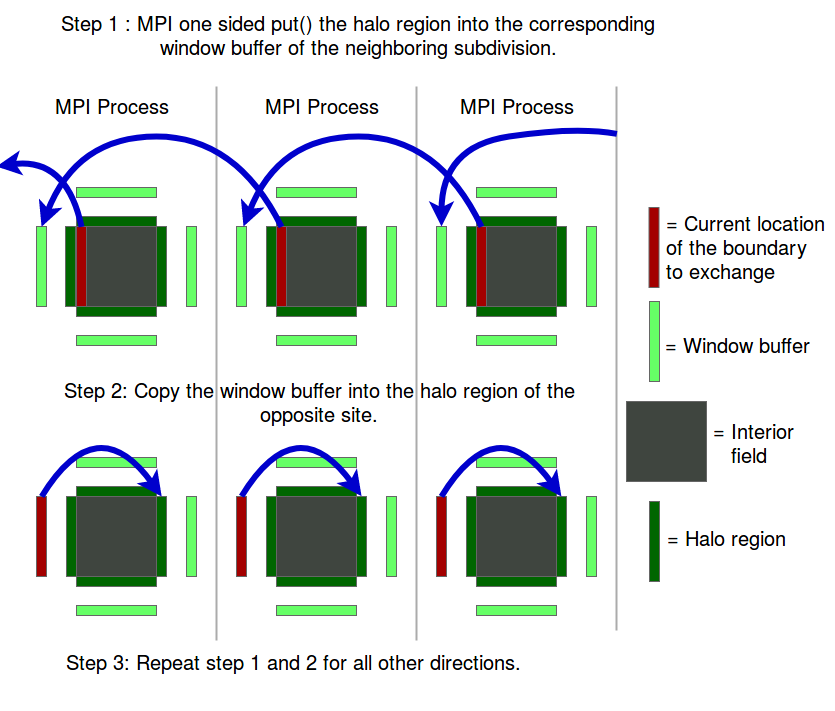
\includegraphics[width=\textwidth]{mpi_onesided.png}
\caption{Schematic representation of the MPI one-sided communication procedure.}
\label{fig:mpi_onesided_communication_flow}
\end{figure}

\subsubsection{Windows as buffers}
The communication procedure described in the section before relies on the MPI one-sided windows as buffers for the transfer and as a result requires an additional copy operation.
An idea to avoid this would be to declare the whole field array as a window.
However, for all but one dimension the halo regions are not contiguous and it does not seem to be supported to \texttt{Put} data into the window in a non-contiguous way.
The MPICH documentation of the \texttt{Put} operation mentions displacements from the start of the window can be provided as an argument, but not a stride for non-contiguous data.
Additionally, the MPI4Py \texttt{Put} function does not even have the displacement as an argument.

Therefore, at least at the moment it seems necessary to use the MPI one-sided windows as a buffer that allows the NumPy \texttt{ascontiguousarray} function and copying using NumPy views to handle the transfer of the halo regions that are non-contiguous in the NumPy array.

\subsubsection{Potential limitations}
Keeping the implementation of the one-sided communication similar to the two-way communication procedure has some limiting effect on the potential for one-way communication.

Specifically, a limitation arises because of limitations on the number of MPI communicators.
Each MPI one-sided window is connected to the communicator given at its construction.
However, each window also internally creates a separate MPI communicator.

As mentioned before, the current implementation requires a MPI one-sided window per direction, per field, and per subdivision.
Most MPI implementations limit the number of MPI communicators to 2048. 
\footnote{See for example the following mailing list thread discussing this limit: https://lists.mpich.org/pipermail/discuss/2016-September/004908.html Accessed 25.9.18}
With this setup the 2048 limitation can be reached very easily for large domains.
For example, a stencil running on 8 nodes with 6 MPI processors per node and 1 subdivision per processor already creates $8 \cdot 6 \cdot 1 \cdot 6 = 288$ windows per field.
In that case, if more than 7 fields are used the MPI communicator limit is reached.

This limitation is accounted for by only creating a MPI one-sided window when it is actually needed e.g. excluding directions with a halo size of 0.

Nevertheless, this limitation can still make it not feasible to use the one-way communication for larger stencil codes.
By designing the one-sided communication procedure to be less similar to the two-way communication and be more optimized for one-sided communication this limitation could be avoided.

